%========== Balanced Binary Search Trees ==========%

\chapter{Balanced Binary Search Trees}
\label{ch:balancedbinarysearchtrees}

\textbf{Pensum} 12 + 13 \cite{clrs} \\\\
\textbf{Relevant Assignment} 13-3 \\\\
\textbf{Algorithms} Red-black tree, AVL-tree \\\\
\textbf{Keywords} ADT, BST structure- and property, rebalance, rotation
\vspace{1in}

\noindent A binary search tree is a node-based data structure that uses
pointers to keep the structure of a a set of nodes intact. Since the data
structure is purely held together by pointers, performing alterations on it
is very fast.
\\\\
\noindent \textbf{Structure} \\
Each node holds a $key$ and three pointers; one for each child-node, $left$
and $right$, and one for its parent-node $p$.
\\\\
\noindent \textbf{Property} \\
Let $x$ be a node in a binary search tree. If $y$ is a node in the left
subtree of $x$, then $y.key \leq x.key$. If $y$ is a node in the right
subtree of $x$, then $y.key \geq x.key$.

\newpage
\section{Searching}
Given the structure of a binary search tree, searching for a particular entry
is at most $O(\lg n)$, assuming that the tree is balanced. Should the tree not
be balanced the worst-case scenario is that the tree only has left- or right-
hand side children, which then produces a list, and searching a list takes
linear time $O(n)$.
 
\section{Insertion}
...

% TODO: prove the run-time.

\section{Deletion}
...

% TODO: prove the run-time

\section{Rotation}
...
\begin{figure}[H]
	\center
	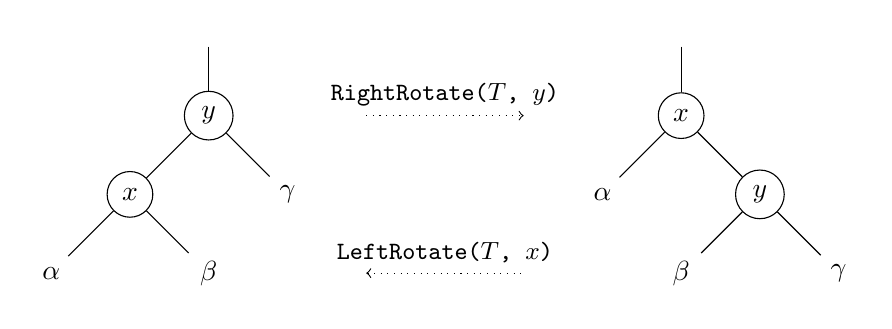
\begin{tikzpicture}
	[
	scale=1.0,
	align=center,
	empty/.style={},
	node/.style={circle, fill=white, draw=black},
	leaf/.style={circle, fill=white}
	]
		% transition
		\draw [->, dotted] (4, 2) -- node [above] {\small \texttt{RightRotate($T$, $y$)}} (6, 2);
		\draw [<-, dotted] (4, 0) -- node [above] {\small \texttt{LeftRotate($T$, $x$)}} (6, 0);
		
		% left
		\node (le) [empty] at 	(2, 3) {};
		
		\node (ly) [node] at 	(2, 2) {$y$};
		\node (lx) [node] at	(1, 1) {$x$};
		
		\node (la) [leaf] at 	(0, 0) {$\alpha$};
		\node (lb) [leaf] at 	(2, 0) {$\beta$};
		\node (lc) [leaf] at 	(3, 1) {$\gamma$};
	
		% right
		\node (re) [empty] at 	(8, 3) {};
		
		\node (ry) [node] at 	(9, 1) {$y$};
		\node (rx) [node] at	(8, 2) {$x$};
		
		\node (ra) [leaf] at 	(7, 1) {$\alpha$};
		\node (rb) [leaf] at 	(8, 0) {$\beta$};
		\node (rc) [leaf] at 	(10, 0) {$\gamma$};	
		% drawing code
		\foreach \from/\to in {le/ly,ly/lx,lx/la,lx/lb,ly/lc} \draw (\from) -- (\to);
		\foreach \from/\to in {re/rx,rx/ra,rx/ry,ry/rb,ry/rc} \draw (\from) -- (\to);
	\end{tikzpicture}
	\caption{Left- and right BST rotations}
	\label{fig:bst-rotations}
\end{figure}
...

% TODO: prove the run-time

\section{Rebalancing}
When we use a balanced implementation of binary search trees, such as
\textit{red-black}- or \textit{AVL}-trees, we must maintain certain
properties, which are typically accounted for after applying an alteration on
the tree - this is called \textit{rebalancing} - whenever a tree gets
unbalanced, as the result of an operation performed on it, we say that the
tree is \textit{left- or right heavy}.

% TODO: write up cases for unbalanced trees, and how to fix them up.
